%Copyright 2014 Jean-Philippe Eisenbarth
%This program is free software: you can 
%redistribute it and/or modify it under the terms of the GNU General Public 
%License as published by the Free Software Foundation, either version 3 of the 
%License, or (at your option) any later version.
%This program is distributed in the hope that it will be useful,but WITHOUT ANY 
%WARRANTY; without even the implied warranty of MERCHANTABILITY or FITNESS FOR A 
%PARTICULAR PURPOSE. See the GNU General Public License for more details.
%You should have received a copy of the GNU General Public License along with 
%this program.  If not, see <http://www.gnu.org/licenses/>.

%Based on the code of Yiannis Lazarides
%http://tex.stackexchange.com/questions/42602/software-requirements-specification-with-latex
%http://tex.stackexchange.com/users/963/yiannis-lazarides
%Also based on the template of Karl E. Wiegers
%http://www.se.rit.edu/~emad/teaching/slides/srs_template_sep14.pdf
%http://karlwiegers.com
\documentclass{scrreprt}
\usepackage{listings}
\usepackage{tabularx}
\usepackage{underscore}
\usepackage[bookmarks=true]{hyperref}
\usepackage[utf8]{inputenc}
\usepackage[portuguese]{babel}
\usepackage[inline]{enumitem}
\usepackage{hyperref}
\usepackage{placeins}
\usepackage[numberedsection]{glossaries}
\usepackage{graphicx}
\setlist[enumerate]{label=(\alph*), nosep, leftmargin=18pt, topsep=-5pt}
\hypersetup{
    bookmarks=false,    % show bookmarks bar?
    pdftitle={INTERFACE, CASOS DE TESTE E MUDANÇA},    % title
    pdfsubject={TeX and LaTeX},                        % subject of the document
    pdfkeywords={TeX, LaTeX, graphics, images}, % list of keywords
    colorlinks=true,       % false: boxed links; true: colored links
    linkcolor=blue,       % color of internal links
    citecolor=black,       % color of links to bibliography
    filecolor=black,        % color of file links
    urlcolor=purple,        % color of external links
    linktoc=page            % only page is linked
}%
\def\myversion{1.0}
\date{}

%}

\newenvironment{enumalfa}[2][label=(\alph*), nosep, leftmargin=19pt, topsep=-5pt]
{
    \begin{minipage}[t]{#2\textwidth}
    \vspace{-9pt}
    \begin{enumerate}[#1]
}
{
    \end{enumerate}
    \vspace{9pt}
    \end{minipage}
}

\newenvironment{enumalfa*}[1][label=(\alph*)]
{\begin{enumerate*}[#1]}
{\end{enumerate*}}

\newenvironment{tabela}[1]
{
    \begin{table}[!htbp]
    \def\arraystretch{1.2}
    \begin{tabular}{#1}
}
{
    \end{tabular}
    \end{table}
}

\usepackage{hyperref}
\makeglossaries

\newglossaryentry{front} {
    name=front-end,
    description={É a parte visual de um software}
}

\newglossaryentry{back} {
    name=back-end,
    description={É a parte de serviços de um software}
}


\newglossaryentry{token} {
    name=token,
    description={É uma identificação}
}

\newglossaryentry{infraAC} {
    name=infra-as-code,
    description={É uma infraestrutura definida por código}
}




\newglossaryentry{prs}{
    name=pull requests,
    description={É quando um desenvolvedor terima uma tarefa e deixa pré encaminhado para subir a alteração}
}

\newacronym{e2e}{e2e}{End-to-end é um código que testa uma funcionalidade por completo}
\begin{document}

\begin{flushright}
    \rule{16cm}{5pt}\vskip1cm
    \begin{bfseries}
        \Huge{INTERFACE, CASOS DE TESTE E MUDANÇA}\\
        \vspace{1.2cm}
        para\\
        \vspace{1.2cm}
        Gerenciador de tarefas\\
        \vspace{1.2cm}
        \LARGE{Versão \myversion}\\
        \vspace{1.2cm}
        Preparado por:  \\Lucas da Silva Santos\\Matheus Zanivan Andrade\\Rafael Nascimento Lourenço\\
        \vspace{1.2cm}
        Senac: Serviço Nacional de Aprendizagem Comercial\\
        \vspace{1.2cm}
        \today\\
    \end{bfseries}
\end{flushright}

\tableofcontents

\chapter{Wireframe}

\begin{figure}[h]
    \centering
    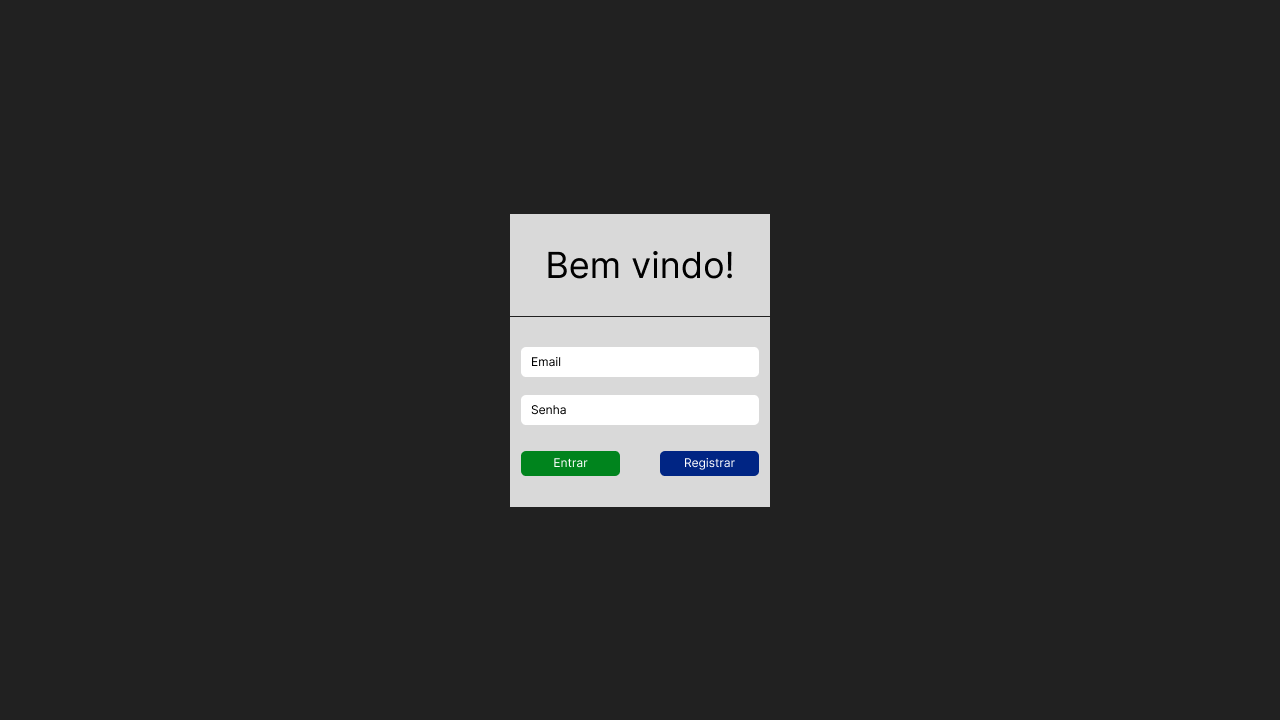
\includegraphics[width=1\textwidth]{../figures/login.png}
    \caption{Tela de login}
    \label{fig:login}
\end{figure}

\begin{figure}[h]
    \centering
    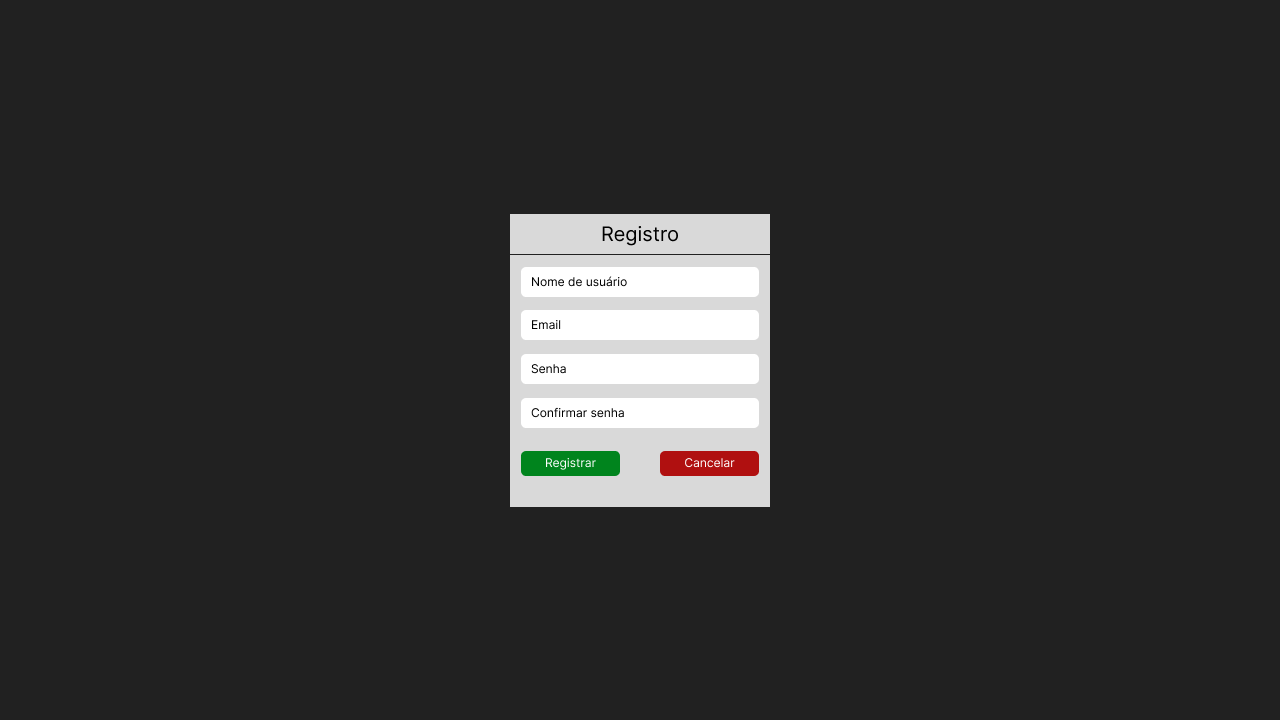
\includegraphics[width=1\textwidth]{../figures/registrar.png}
    \caption{Tela de registro de usuário}
    \label{fig:registrar}
\end{figure}

\begin{figure}[h]
    \centering
    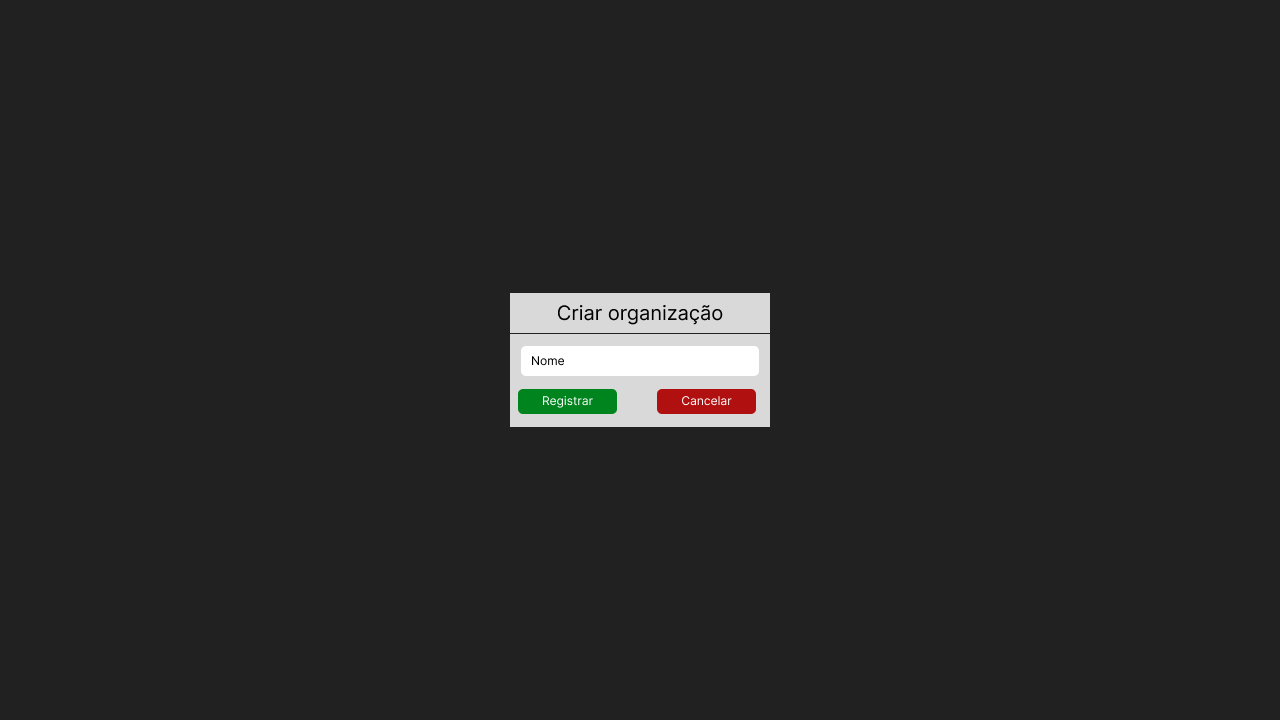
\includegraphics[width=1\textwidth]{../figures/criar-organizacao.png}
    \caption{Tela de criar organização}
    \label{fig:criar-organizacao}
\end{figure}

\begin{figure}[h]
    \centering
    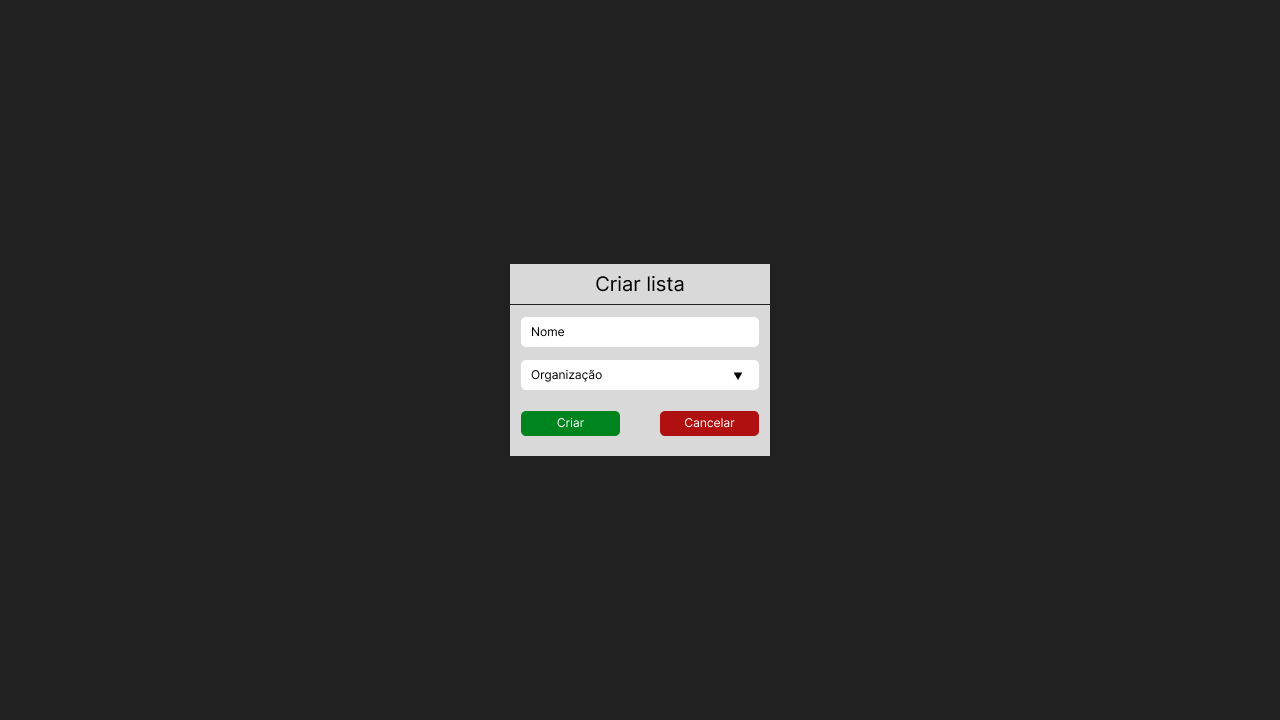
\includegraphics[width=1\textwidth]{../figures/criar-lista.png}
    \caption{Tela de criar lista de tarefas}
    \label{fig:criar-lista}
\end{figure}

\begin{figure}[h]
    \centering
    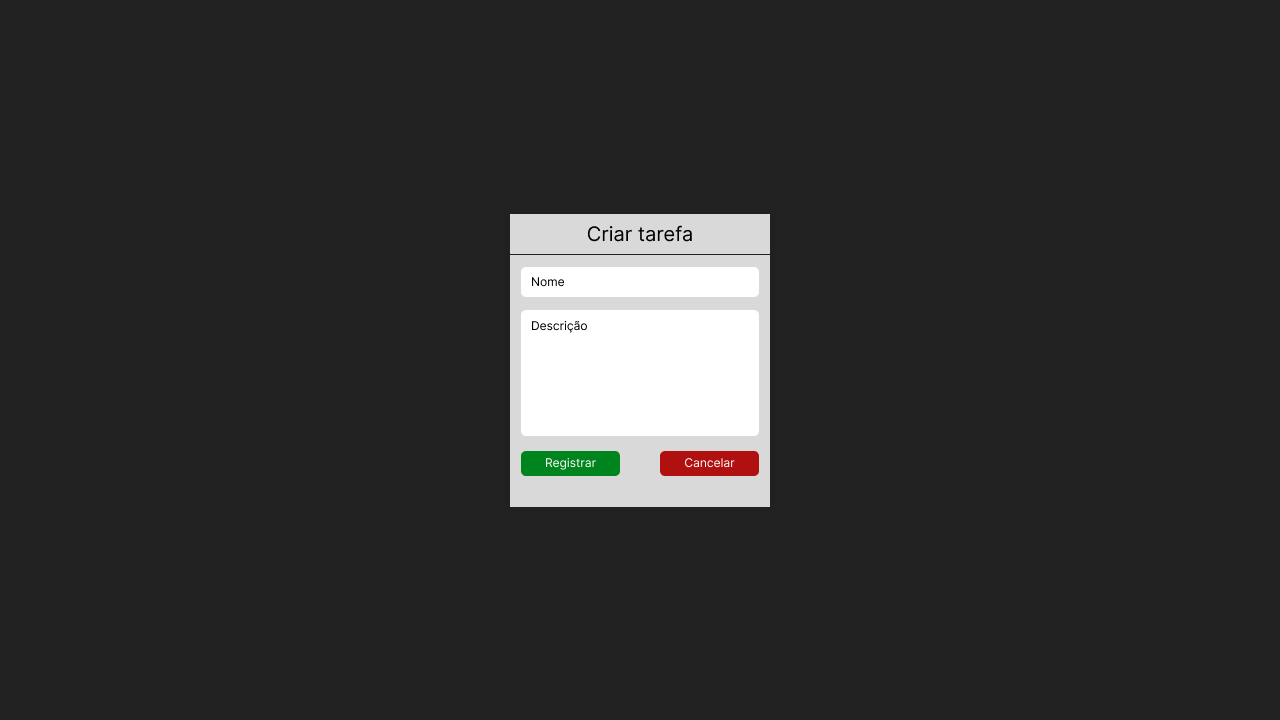
\includegraphics[width=1\textwidth]{../figures/criar-tarefa.png}
    \caption{Tela de criar tarefas}
    \label{fig:criar-tarefa}
\end{figure}

\chapter{Plano de testes}

    \begin{tabularx}{\textwidth}{|X|X|}
        \hline
        Seção & Descrição \\
        \hline
        Identificador do Plano de Teste & Plano de Teste para a Funcionalidade de gerenciamento de tarefas. \\
        \hline
        Introdução & Este plano de teste tem como objetivo garantir o correto funcionamento do recurso de gerenciamento de tarefas em nosso aplicativo de gerenciamento de tarefas. \\
        \hline
        Itens de Teste & A funcionalidade de tarefas do aplicativo. \\
        \hline
        Funcionalidades a serem Testadas & Criar, deletar e editar as tarefas devem conter as mesmas informações no contexto do usuário e no banco de dados ápos a confirmação da ação. \\
        \hline
        Funcionalidades que não serão Testadas & Funcionalidades não relacionadas à tarefas do aplicativo. \\
        \hline
        Abordagem & Usaremos testes manuais \acrshort{e2e}. Portanto criaremos testes que irão checar o fluxo por completo, em cada parte terá uma validação da resposta. O fluxo será criar uma tarefa, seguido de editar essa tarefa e depois deleta-lá. \\
        \hline
        Critérios de Aprovação/Falha do Item & Todas as etapas serão validadas e se alguma falhar o teste inteiro irá parar com uma mensagem de erro especificando onde parou. As checagens serão uma comparação direta entre as mudanças de estado entre o aplicativo e o banco de dados. \\
        \hline
        Necessidades Ambientais & Os testes serão realizados em dispositivos Android e iOS, com várias versões de cada sistema operacional e diferentes tamanhos de tela. \\
        \hline
        \end{tabularx}

        \begin{tabularx}{\textwidth}{|X|X|}
            \hline
            Seção & Descrição \\
            \hline
            Identificador do Plano de Teste & Plano de Teste para a Funcionalidade de criação de usuários. \\
            \hline
            Introdução & Este plano de teste tem como objetivo garantir o correto funcionamento do recurso de criação de usuários em nosso aplicativo de mensagens. \\
            \hline
            Itens de Teste & A funcionalidade de criar usuários do aplicativo. \\
            \hline
            Funcionalidades a serem Testadas & Criar usuários deve conter as mesmas informações no contexto do usuário e no banco de dados ápos a confirmação da ação. \\
            \hline
            Funcionalidades que não serão Testadas & Funcionalidades não relacionadas à usuários do aplicativo. \\
            \hline
            Abordagem & Usaremos uma bateria de testes manuais com um banco de dados em memória visto que terá várias condições para criar o usuário, utilizaremos a ferramenta H2 para subir o bando de dados em memória. Os testes irão abranger todos as condições relacionadas a singularidade do e-mail e a senha. Ou seja, além de criar o usuário e validar no banco de dados, será validado os outros os casos nos quais terão que retornar erro como resposta certa. \\
            \hline
            Critérios de Aprovação/Falha do Item & Todas as etapas serão validadas e se alguma falhar o teste inteiro irá parar com uma mensagem de erro especificando onde parou. Sempre validando em cada etapa as alterações do contexto do usuário e do banco de dados. \\
            \hline
            Necessidades Ambientais & Os testes serão realizados em dispositivos Android e iOS, com várias versões de cada sistema operacional e diferentes tamanhos de tela. \\
            \hline
        \end{tabularx}

        \begin{tabularx}{\textwidth}{|X|X|}
                \hline
                Seção & Descrição \\
                \hline
                Identificador do Plano de Teste & Plano de Teste para a Funcionalidade de gerenciamento de lista de tarefas. \\
                \hline
                Introdução & Este plano de teste tem como objetivo garantir o correto funcionamento do recurso de gerenciamento de lista de tarefas em nosso aplicativo de gerenciamento de tarefas. \\
                \hline
                Itens de Teste & A funcionalidade de lista de tarefas do aplicativo. \\
                \hline
                Funcionalidades a serem Testadas & Criar, deletar e editar as lista de tarefas devem conter as mesmas informações no contexto do usuário e no banco de dados ápos a confirmação da ação. Além de um teste de erro que deverá validar o retorno impossibilitando uma inserção de lista de tarefas com o mesmo nome dentro da organização que se encontra.\\
                \hline
                Funcionalidades que não serão Testadas & Funcionalidades não relacionadas à lista de tarefas do aplicativo. \\
                \hline
                Abordagem & Usaremos testes manuais \acrshort{e2e}. Portanto criaremos testes que irão checar o fluxo por completo, em cada parte terá uma validação da resposta. O fluxo será criar uma lista de tarefas, seguido de editar essa lista de tarefas e depois deleta-lá. Depois será testado o caso de tentar criar uma lista de tarefa com nome duplicado na mesma organização, o que deve retornar erro.\\
                \hline
                Critérios de Aprovação/Falha do Item & Todas as etapas serão validadas e se alguma falhar o teste inteiro irá parar com uma mensagem de erro especificando onde parou. As checagens serão uma comparação direta entre as mudanças de estado entre o aplicativo e o banco de dados.\\
                \hline
                Necessidades Ambientais & Os testes serão realizados em dispositivos Android e iOS, com várias versões de cada sistema operacional e diferentes tamanhos de tela. \\
                \hline
            \end{tabularx}

\chapter{Teste de Carga}


\section*{Objetivo do teste}
Esse teste de carga tem o objetivo de avaliar se um aplicativo de gerenciamento de tarefas tem a capacidade de suportar simultaneamente 20000 usuários sem perder desempenho.

\section*{Escopo do Teste}

No aplicativo, serão realizados testes nos seguintes campos:

\begin{itemize}
    \item Criação de usuários: O objetivo é determinar a quantidade de usuários que podem ser criados simultaneamente, bem como a capacidade total de criação de usuários.
    \item Gerenciamento de sessão: Será simulada a presença de múltiplos usuários simultâneos na aplicação, a fim de verificar a capacidade de gerenciamento de sessões.
    \item Listas: Será avaliada a capacidade de criação e exclusão de listas, buscando determinar a quantidade máxima de listas que podem ser criadas e removidas com sucesso.
    \item Criação de tarefas: Será testada a capacidade de criação e exclusão de tarefas, com o intuito de verificar o limite de tarefas que podem ser criadas e removidas.
\end{itemize}

\section*{Cenário de teste}
Para simular a carga e o tráfego deste aplicativo, utilizaremos a ferramenta Loadview. Essa ferramenta nos permite simular a quantidade de usuários simultâneos, avaliar o desempenho, escalabilidade, identificar os limites, a estabilidade e garantir a qualidade do aplicativo. Serão simulados 30.000 usuários simultâneos para assegurar o funcionamento adequado da aplicação acima da capacidade esperada, sem perda de desempenho. Dentre os 30.000 usuários simulados, 15.000 serão destinados a testar o gerenciamento de sessões, entrando e saindo do aplicativo, enquanto os outros 15.000 irão navegar entre a tela de lista de tarefas e as tarefas.

E para testar a quantidade de dados que a aplicação deve lidar serão criadas 30000 mil contas distintas, e cada uma das contas criadas terão uma organização atrelada com o nome e uma lista de tarefas contendo 3 tarefas.

\section*{Métricas para coletar}
Durante os testes, serão coletados dados como o tempo de resposta, a taxa de erros, a utilização de recursos, a concorrência, o tempo de carregamento da página e o tempo de conexão.

\section*{Análise dos Resultados}

Ao final da simulação, caso o aplicativo não suporte a carga, faremos uma nova simulação com 25.000 usuários para nos aproximarmos ainda mais da quantidade esperada. Se, mesmo assim, a aplicação não for capaz de suportar essa carga, realizaremos melhorias nos servidores antes de prosseguir com os novos testes. Caso tudo funcione normalmente, o aplicativo de gerenciamento de tarefas será publicado e estará pronto para uso.

\chapter{Gestão de mudança}
Um grupo de empresários compraram uma parte significativa da empresa e decidiu-se criar uma assinatura para a ferramenta em prol de ser mais rentável como negócio. Algumas restrições serão criadas em algumas funcionalidades, isso gerará uma mudança no banco de dados para classificar os usuários com assinatura e sem assinatura além de ter um sistema para pagamentos. 

\section*{Impacto da Mudança}
É uma mudança de grande impacto porque irá abranger várias telas, serviços, condições e mensagens de erro. Segue as limitações.

\subsection*{Usuários sem assinatura poderão criar apenas uma organização}
Essa condição terá que validar se o usuário logado possui assinatura antes de efetuar a ação e a tela na qual se cria a organização terá que ser revisada para facilitar o entendimento dessa nova restrição.

\subsection*{Usuários sem assinatura poderão criar apenas cinco listas de tarefas}
Essa condição terá que validar se o usuário logado possui assinatura antes de efetuar a ação e a tela na qual se cria a lista de tarefas terá que ser revisada para facilitar o entendimento dessa nova restrição.

\subsection*{Usuários sem assinatura poderão criar no máximo três tarefas por dia}
Essa condição terá que validar se o usuário logado possui assinatura antes de efetuar a ação e a tela na qual se cria tarefas terá que ser revisada para facilitar o entendimento dessa nova restrição.

\subsection*{Uma organização com um dono sem assinatura não poderá ter mais de cinco colaboradores ativos}
Essa condição terá que validar se o usuário dono na organização possui assinatura antes de efetuar a ação e a tela na qual se atribui usuários à organização terá que ser revisada para facilitar o entendimento dessa nova restrição.

\subsection*{Novo módulo de pagamento}
Esse módulo será atrelado ao módulo de assinatura na qual permiitirá ao usuário adicionar um cartão de crédito para as bandeiras solicitadas em prol de ativar a assinatura.

\subsection*{Novo módulo para visualização dos resultados das listas de tarefas}
Esse módulo será atrelado a listas de tarefas para auxiliar o dono do projeto com métricas de progresso da equipe, possibilitando uma visão geral do desempenho semanal, mensal e anual de cada colaborador da empresa.
 Esse novo módulo será apenas para donos de organizações com assinatura.

\section*{Comunicação da Mudança}
A mudança será notificada para todos usuários por e-mail, notificação duas vezes sendo elas, uma vez antes de ocorrer a mudança e no próprio dia da mudança. Outra notificação será exibida na primeira vez que o usuário abrir o aplicativo. 

A mensagem que será passada aos usuários é um aviso sobre as mudanças que ocorerrão, que visam arrecadar contribuidores para criar novas funcionalidades e garantir uma qualidade melhor de entregas. Possibilitando contratar novos funcionários que irão gerenciar a parte de testes e correção de erros de forma mais rápida.

\section*{Medição do Sucesso da Mudança}
O sucesso será medido com número de erros reportados nos três primeiros meses e a taxa de aprovação dos clientes de curto e longo prazo. 

\subsection*{Erros reportados}
Será criada um sistema de pontuação para mensurar o sucesso da mudança, caso ápos três meses a pontuação do sistema de pontos baseados em erros seja abaixo de 25  pontos então obteve-se sucesso na mudança, o sistema de pontos será definido com: 
\subsubsection*{Erros de alta prioridade}
Maneiras de burlar a condições de assinatura ou problemas no sistema de pagamento. Cada problema diferente reportado somará 10 pontos. 

\subsubsection*{Erros de prioridade média}
 Erros inesperados em contextos nos quais eram para funcionar a ação. Cada problema diferente reportado somará 5 pontos. 
 
\subsubsection*{Erros de baixa prioridade}
Erros relacionados a parte visual do projeto. Cada problema diferente reportado somará 2 pontos.

\subsection*{Taxa de aprovação dos clientes}
Em curto prazo se espera que tenha uma aceitação e assinatura de 20\% do público o que seria nesse período de três meses. A longo prazo — 1 ano — se pretende aumentar o número total de assinantes para 50\% do público atual.


\printglossary

\end{document}